\section{Problem Definition}

Website loading speed has a critical impact on page abandonment rate among its visitors. According to a Google experiment, website loading time worsened only by \textbf{half of a second} had a 20\% drop in its visitor’s traffic. \cite{KISSmetrics:Speed-Google} From the figure \ref{fig:kissmetrics-page-abandonment} \cite{Fig:Kissmetrics-page-abandonment}, we can see a chart of page abandonment relative to a web page loading time in seconds. By the time a ten-second-long web page is loaded to its visitors, more than 35\% of them will close the page, never seeing what is on it.

\begin{figure}[H]
\begin{center}
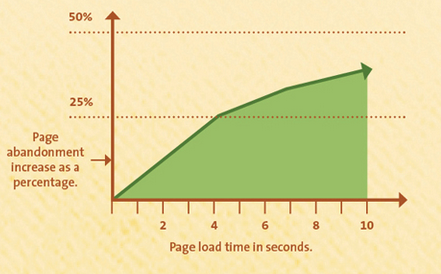
\includegraphics[scale=0.5]{figures/page-abandonment-chart.png}
\caption{Slower page response time results in an increase in page abandonment}
\label{fig:kissmetrics-page-abandonment}
\end{center}
\end{figure}

To highlight the seriousness of this issue, imagine a situation in which an e-commerce site owner is making \$100,000 per day. One-second page delay could potentially cost him or her \$2.5 million in lost sales every year \cite{Fig:Kissmetrics-page-abandonment}. See figure \ref{fig:kissmetrics-eshop-delay} for more detail.

\begin{figure}[H]
\begin{center}
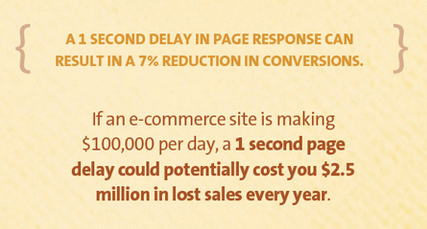
\includegraphics[scale=0.5]{figures/kissmetrics-eshop-delay.png}
\caption{What can a one-second page delay cause to your e-commerce site?}
\label{fig:kissmetrics-eshop-delay}
\end{center}
\end{figure}

What is more, Google incorporated site speed in search rankings in 2010 \cite{MattCutts:Google-site-speed-seo}, meaning that the more time it takes to load a website, the lower it ranks in Google search results. We believe we have shown the reader enough evidence that optimizing the performance and speed of a website is crucial for its success, especially in today's fast-paced world.

\section{About WordPress}

\subsection{General Information}

Citing WordPress.org, "WordPress is web software you can use to create a beautiful website or blog."\cite{WP:WP.org} Simply put, WordPress is a powerful, open-source web publishing software, content management system and a web platform for building rich web applications. People and companies use WordPress for various purposes and reasons, most notably for their blogs, websites, e-commerce solutions and large web portals. At the time of writing, it is estimated that about 24\% \cite{W3Techs:WP-usage} of all websites, whose content management system is known, are being run on WordPress. This number is rather astonishing because it means that visiting five random websites, one of them will be a WordPress-powered one. \\

WordPress, in comparison to other web software and frameworks, is a full-featured, stand-alone web publishing software and content management system. WordPress is written mostly in PHP language, accompanied with JavaScript scripts and CSS stylesheets. At its core, it consists of a request-response routing subsystem, classes for managing database and content, security features and others. Initially, WordPress was started as an open-source hobby project of Matt Mullenweg in 2003 \cite{WP:History}. Since then, web programmers from all around the world have contributed to it, making it robust, secure and fast. However, as there are several bottlenecks in the system, we, web developers, decided to analyze and improve them. Our findings and results are summarized in this thesis.

\subsection{WordPress-Powered Website}

In order to customize the look and feel of user’s instance of the website, there exists a mechanism called the WordPress Theme. A WordPress theme is simply a collection of scripts, stylesheets and images which get combined, processed and the generated content is sent back to the client. A user can install any theme which is compatible with his or her WordPress version. There is no central body governing the quality and correctness of a theme. As theme developers are free to build them almost arbitrarily, numerous security and performance flaws occur. The WordPress Plugin is a pluggable piece of software which enhances the basic WordPress functionality, thus enabling its users to heavily modify their WordPress-based web applications and sites. Plugins are also open source and without any quality guarantees, therefore experiencing the same problems as the aforementioned themes. \\

Moreover, when a user has a high-traffic website, his web delivering server is not able to keep up with all the requests resulting in a slow, unresponsive website. The reader might assume that the problems would be solved by increasing plugins quality. While the previous statement is true, it is usually not viable, mainly due to a reason that work of an experienced web developer is relatively expensive. In many cases, upgrading the server and/or getting additional one(s) is the preferred way. In our work, we are concerned with optimizing the server software first and only then examining the best practices, tips and tricks of a plugin or a theme development.

\section{General Techniques for Improving Website Loading Speed}

Before we can delve into solutions to our problems, we need to list and describe several general techniques and measures used to improve not only the website loading times, but also a server resources usage and load.

\subsection{Web-Serving Software Efficiency}

Using the most performant and the least resource-hungry web-serving software is usually the most effective way of improving web page loading speed. Some studies have found that even small changes to configuration files can a difference. In our work, we are making comparisons between the two most popular web-serving applications, namely Apache HTTP and Nginx, as well as comparisons between different PHP interpreters. Jump to section \ref{sec:nginx-apache} for more details and statistics. 

\subsection{Server-Side Caching}

Let us divide server-side \gls{caching} into three main categories:

\begin{enumerate}
    \item\textbf{Caching intermediate PHP code}
    \item\textbf{Caching the output of PHP interpreter (so called “page cache”)}
    \item\textbf{Static resources (files) caching}
    \item\textbf{Database caching}
  \end{enumerate}

\subsection*{Caching intermediate PHP code}

PHP source code is interpreted on each run, thus the PHP interpreter has to read and collect all required files each time a new request is sent to our WordPress-based website. With PHP opcode caching, an intermediate source code is generated on the first run and stored temporarily. When a new request comes, instead of going through all the files, PHP loads cached opcode and executes it. We can observe the process from the figure \ref{fig:php-opcode-caching} \cite{Fig:PHP-opcode-caching}.

\begin{figure}[H]
\begin{center}
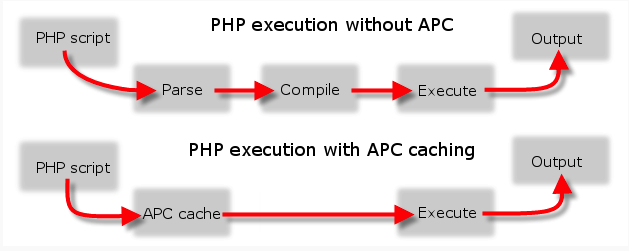
\includegraphics[scale=0.5]{figures/php-opcode-caching.png}
\caption{PHP execution diagram with and without APC opcode cache.}
\label{fig:php-opcode-caching}
\end{center}
\end{figure}

\subsection*{Caching the output of PHP interpreter (so called “page cache”)}

While a website based on WordPress is dynamic, in some cases it is possible to store the constructed web page for subsequent usage. This process is usually called page caching and it is suitable for websites with static blocks of content. However, problems arise when we have to handle special cases such as when a visitor is logged into our website. In that case, we are not able to cache the request because other visitors would see the logged-in visitor’s cached content instead of a general one.

\subsection*{Static resources (files) caching}

When our website consists of a large number of (smaller) files such as JavaScript scripts, CSS stylesheets, images and others, caching these resources is an idea worth mentioning. They are constructed and loaded on the initial request, stored in a local web server cache and retrieved from the cache on subsequent requests.\\ 

The largest disadvantage of static file caching is usually a drop in free memory available to different needs of the web server, especially when files are cached in RAM memory.

\subsection*{Database caching}

When multiple requests to our web server trigger the same database queries, it is reasonable to store the retrieved data for later use. When a subsequent request is made, querying the database is omitted, thus preserving valuable server resources and outputting the resulting web page faster.

\subsection{Client-Side Caching}

What makes client-side caching different from the server-side caching is that data is stored locally in the visitor’s browser, not on the server to which the requests are made. \cite{Study:Mnot-caching} The whole hypertext document with all its resources including JavaScript scripts and CSS stylesheets can get cached in client's browser storage, loaded from it on consecutive requests. Naturally, the most notable advantage of client-side caching is the fact that the user’s browser does not need to download the locally cached resources. \\

On the other hand, we need to implement a mechanism which can handle resource changes on the server-side. When not done properly, some of the visitors might see outdated content due to the reason that the visitor’s browser has not been instructed to revalidate its cache.

\subsection{JavaScript and CSS Resource Minification and Combination}

At the time of writing (early 2015), a large number of WordPress themes and plugins contain tens or more JavaScript scripts and CSS styles, especially the more professional ones. It is caused by the fact that users like having amazingly looking, feature-rich websites. The problem with this fact is twofold:
 
\begin{itemize}
	\item \textbf{There is a limit on the number of concurrent downloads of resources from the same domain. Both Internet Explorer 8 and Google Chrome allow six concurrent downloads while Firefox eight. \cite{SO:Browser-concurrent-downloads}}
	\item \textbf{Each request carries an overhead of constructing a HTTP packet, sending it to the web server and waiting for the reply.}
\end{itemize}

There are two well-known methods of solving this issue:

\begin{enumerate}
    \item\textbf{Resources combination and/or}
    \item\textbf{resources minification.}
  \end{enumerate}

\subsection*{Resources combination}

Resource combination is a process in which resources on the requested web page are collected into (preferably) single file which is then sent back to the visitor’s browser. There exist two main downsides of this approach. The first is that collecting the resources consumes additional CPU cycles on the server-side. Another disadvantage happens when the owner of the website modifies source code of any of the grouped resource. The whole group has to be gathered together again, including revalidating browser cache if present.

\subsection*{Resources minification}

JavaScript scripts and CSS stylesheets can be minified. Minification is a procedure in which parts of a script or a stylesheet are reduced or completely removed, thus reducing its size and length. Advanced minification tools are capable of refactoring them in a manner that they become even more compact.

\subsection{Compression of Images, HTML and Other Resources}

\subsection*{Image compression}

Images, particularly those produced by the JPEG lossy compression mechanism, can be compressed further, thus reducing their size while keeping a tolerable quality of picture details. At the time of writing this work, the cost of satisfying WordPress plugin \cite{WP-Plugin:EWWW-Image-Optimizer} for image compression is zero.

\subsection*{Hypertext documents and other text-based assets compression}

Before the data is sent back in a response to visitor’s request, its size can be reduced further with a process called data compression. \cite{Study:Google-compression} Most modern web browsers \cite{Study:SO-gzip-browser-support} support GZIP compression of textual data. One of the downsides of performing this process is that additional CPU cycles on both server and client sides are expended in order to compress and uncompress the data.

\subsection{Optimizing Images — Image Sprites}

Images used for our website's user interface as well as other images can become more optimized for use in the web environment. A mechanism called image spriting \cite{Study:CSSwizardy-image-spriting} is a procedure during which multiple images, sometimes even all of them, get collected and combined into a single larger image — sprite. When a web page is requested, instead of loading tens of user interface icons and images, only this single one is sent back to the user, thus saving additional HTTP requests and bandwidth. When rendering the user interface, icons and images are taken from that single image.

\subsection{CDN and Resource Distribution}

In some cases, our website is accessed from many different countries, even continents. If we have web servers located only locally, additional milliseconds start to congregate in these situations. To solve this problem, web administrators usually distribute the website’s data across multiple servers positioned in multiple places around the world. CDN services greatly reduce the amount of work needed to accomplish the goal by doing it automatically for us.

Another quite useful concept is called load balancing. It is a method of distributing requests to a website across multiple web servers decreasing the overall load on each machine.

\section{Similar Studies}

In this section, we will be analyzing and discussing similar studies done by other web developers and programmers. Before we look at their results, we need to have a basic understanding of the web serving software they were comparing. \\

\textbf{Apache HTTP}, also called Apache, is a free and open source world's most widely used (57.5\%\cite{Apache:Usage} of all websites whose web server we know) web server software. \textbf{Nginx}, released nearly 10 years later than Apache, was designed with a high concurrency, high performance and low memory usage in mind, specifically to solve the C10K problem \cite{Nginx:c10k}. \\

Both \textbf{PHP} and \textbf{HHVM} are PHP script interpreters. HipHop Virtual Machine (HHVM), released by Facebook in 2011, was developed to increase the performance of PHP script execution on the Facebook site. Both of them are open source and free to use.

\subsection{Using Nginx, Apache, APC and Varnish in Different Scenarios — Garron.me}

Guillermo Garron, the author of the work \cite{Study:Perf-Garron}, has performed several comparisons between the most popular web-serving and caching software. He used a relatively weak web server with highly limited computing power — 512MB RAM, a shared CPU and a shared disk. However, the result of his experiment is clear — caching the output of the PHP interpreter has a considerable impact on loading times of WordPress-powered web page. \\

From the figure \ref{fig:garron-no-cache}, we observe that if the number of simultaneous visitors exceeds ten, response times of the web server start to dramatically decrease in a linear fashion. On the other hand, response times start to worsen only after thirty concurrent visitors, as we can see from the figure \ref{fig:garron-apc-cache}.

\begin{figure}[H]
\begin{center}
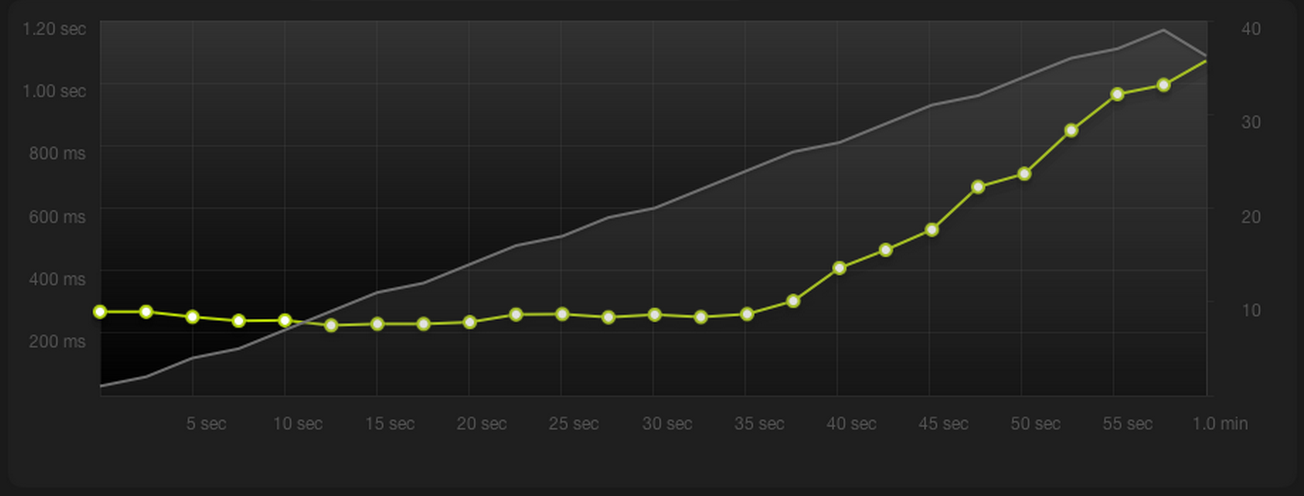
\includegraphics[scale=0.5]{figures/garron-no-cache.png}
\caption{Apache HTTP + PHP, no opcode caching}
\label{fig:garron-no-cache}
\end{center}
\end{figure}

\begin{figure}[H]
\begin{center}
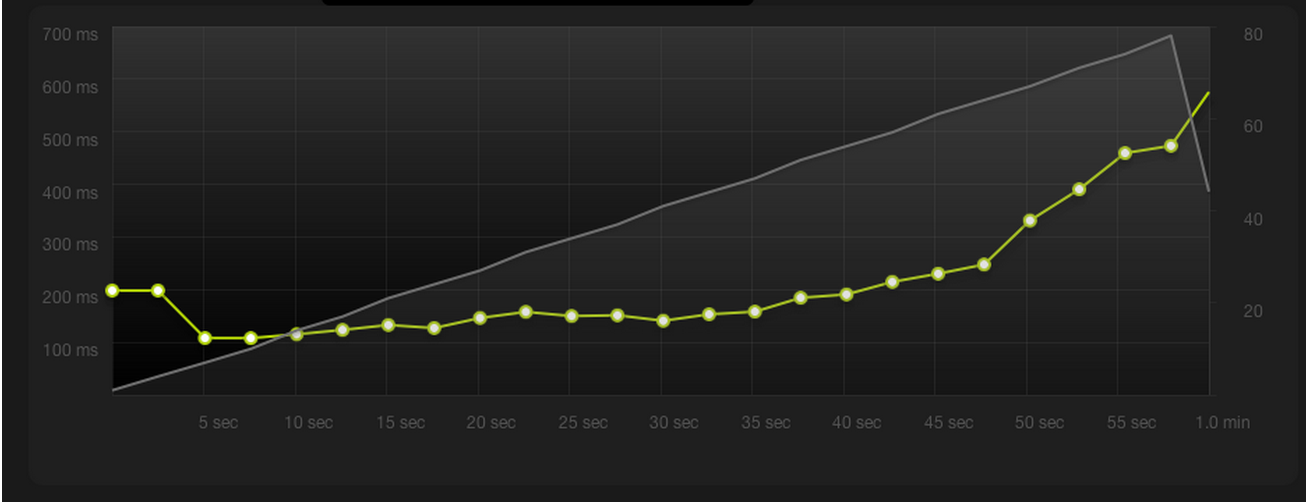
\includegraphics[scale=0.5]{figures/garron-apc-cache.png}
\caption{Apache HTTP + PHP, APC opcode caching}
\label{fig:garron-apc-cache}
\end{center}
\end{figure}

Although using Nginx instead of Apache HTTP yields additional performance gains, they are less notable. Nginx strengths are demonstrated when a website is composed of many resources. However, Garron used a standard WordPress installation, with no extra plugins or complex custom themes.

\subsection{WordPress on HHVM vs WordPress on PHP-FPM — WPengine.com}
\label{sec:WPengine-study}

WPengine.com is a company specializing in offering WordPress web hosting services. They have introduced a new hosting plan which differentiates itself from others by using HHVM PHP interpreter instead of the standard PHP. Before releasing the hosting plan, a study, in which the performance of HHVM versus PHP was compared, was undertaken. The study concluded with a fact that HHVM increased the speed of their servers by 600\% \cite{Study:Perf-WPEngine}. This fact is displayed in the figure \ref{fig:wpengine-hhvm-php-wordpress}.

\begin{figure}[H]
\begin{center}
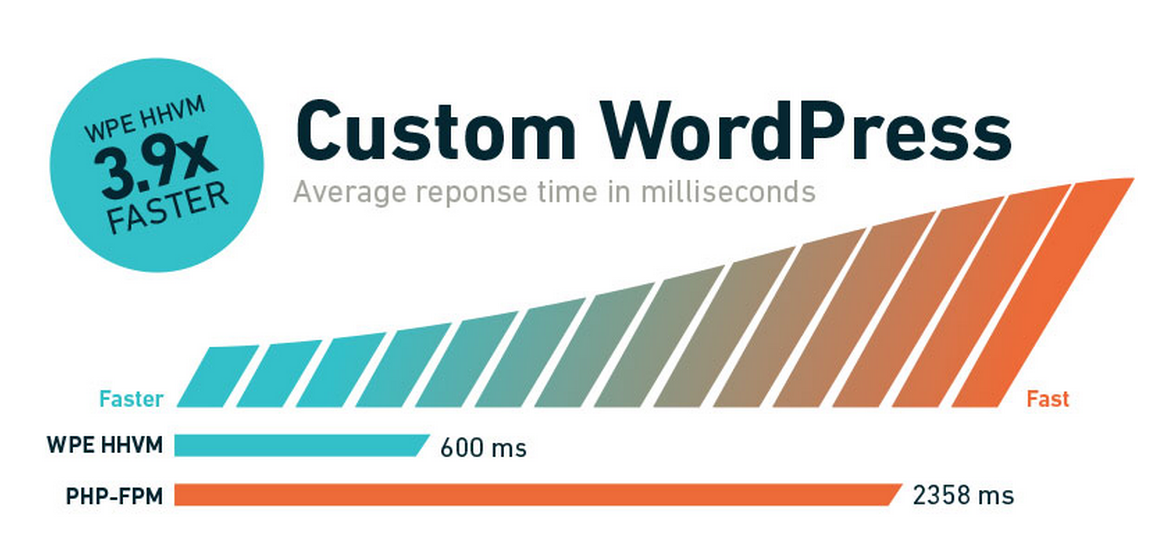
\includegraphics[scale=0.5]{figures/wpengine-hhvm-php-wordpress.png}
\caption{WordPress on PHP vs WordPress on HHVM response times}
\label{fig:wpengine-hhvm-php-wordpress}
\end{center}
\end{figure}

In the study, they found out that HHVM is not 100\% stable yet and occasionally stops working. Their solution to this problem was to redirect the incoming requests to a fallback PHP interpreter while HHVM gets restarted. 

\subsection{WordPress HHVM vs PHP — xyu.io}

Xiao Yu, a web developer, benchmarked \cite{Study:Perf-XYU.io} WordPress running on PHP vs WordPress running on HHVM. His findings show a similar pattern to the findings of WPengine.com in section \ref{sec:WPengine-study}. Outcome of his experimentation can be observed in table \ref{tab:xyu.io-experiment-results}. 

\begin{table}[H]
\begin{tabular}{llll}
                   & \textit{Response Time} & \textit{Ok Responses} & \textit{Errors / Timeouts} \\
\textbf{Anon PHP}  & 4.091                  & 8,939                 & 0.94\%                     \\
\textbf{Anon HHVM} & 2.122                  & 18,308                & 0.00\%                     \\
\textit{Change}    & 48.1\%                 & \textbf{2.05X}        &                            \\
\textbf{Auth PHP}  & 20.688                 & 457                   & 74.17\%                    \\
\textbf{Auth HHVM} & 14.359                 & 1,242                 & 43.45\%                    \\
\textit{Change}    & 30.6\%                 & \textbf{2.72X}        &                           
\end{tabular}
\caption{WordPress on HHVM vs WordPress on PHP — xyu.io}
\label{tab:xyu.io-experiment-results}
\end{table} 
"In the numbers above anonymous requests represents hits to various pages without a WordPress logged in cookie which are eligible for Batcache caching whereas authorized requests are hits to the same pages with a login cookie thus bypassing page caching."\cite{Study:Perf-XYU.io}


